% !TEX root = ../thesis.tex
\section{Usage Scenario}

\emph{Dissecting a Trailer}~\cite{nytimes:trailer} is a visualization from The
New York Times that illustrates how scenes from five Best Picture Oscar nominees
were edited into trailers. It is an example of a visualization that cannot be
built using existing chart typologies or high-level grammars. The visualization
layers several mark types and uses a non-standard ``scatter'' plot with small
rectangles of varying widths. The original consists of over 350 lines of
JavaScript/D3~\cite{bostock:d3} code. Here, we demonstrate how this graphic can
be created using Lyra (Fig.~\ref{fig:lyra:usage}).

\begin{figure}[h!]
\floatbox[{\capbeside\thisfloatsetup{capbesideposition=
{right,center},capbesidewidth=0.3\columnwidth}}]{figure}[\FBwidth]
{\caption{Using Lyra to recreate the New York Times' Dissecting a Trailer.
(a)~Drag a line \emph{mark} onto the canvas. (b)~Drag a field from a
\emph{pipeline}'s data table to a \emph{drop zone} to map it to a mark property.
(c)~Add a ``group by'' \emph{data transform} to create a hierarchy. (d)~Edit a
\emph{scale} definition to reverse the range. (e)~Use a \emph{connector} to
anchor text marks to the rectangles.}
\label{fig:lyra:usage}}
{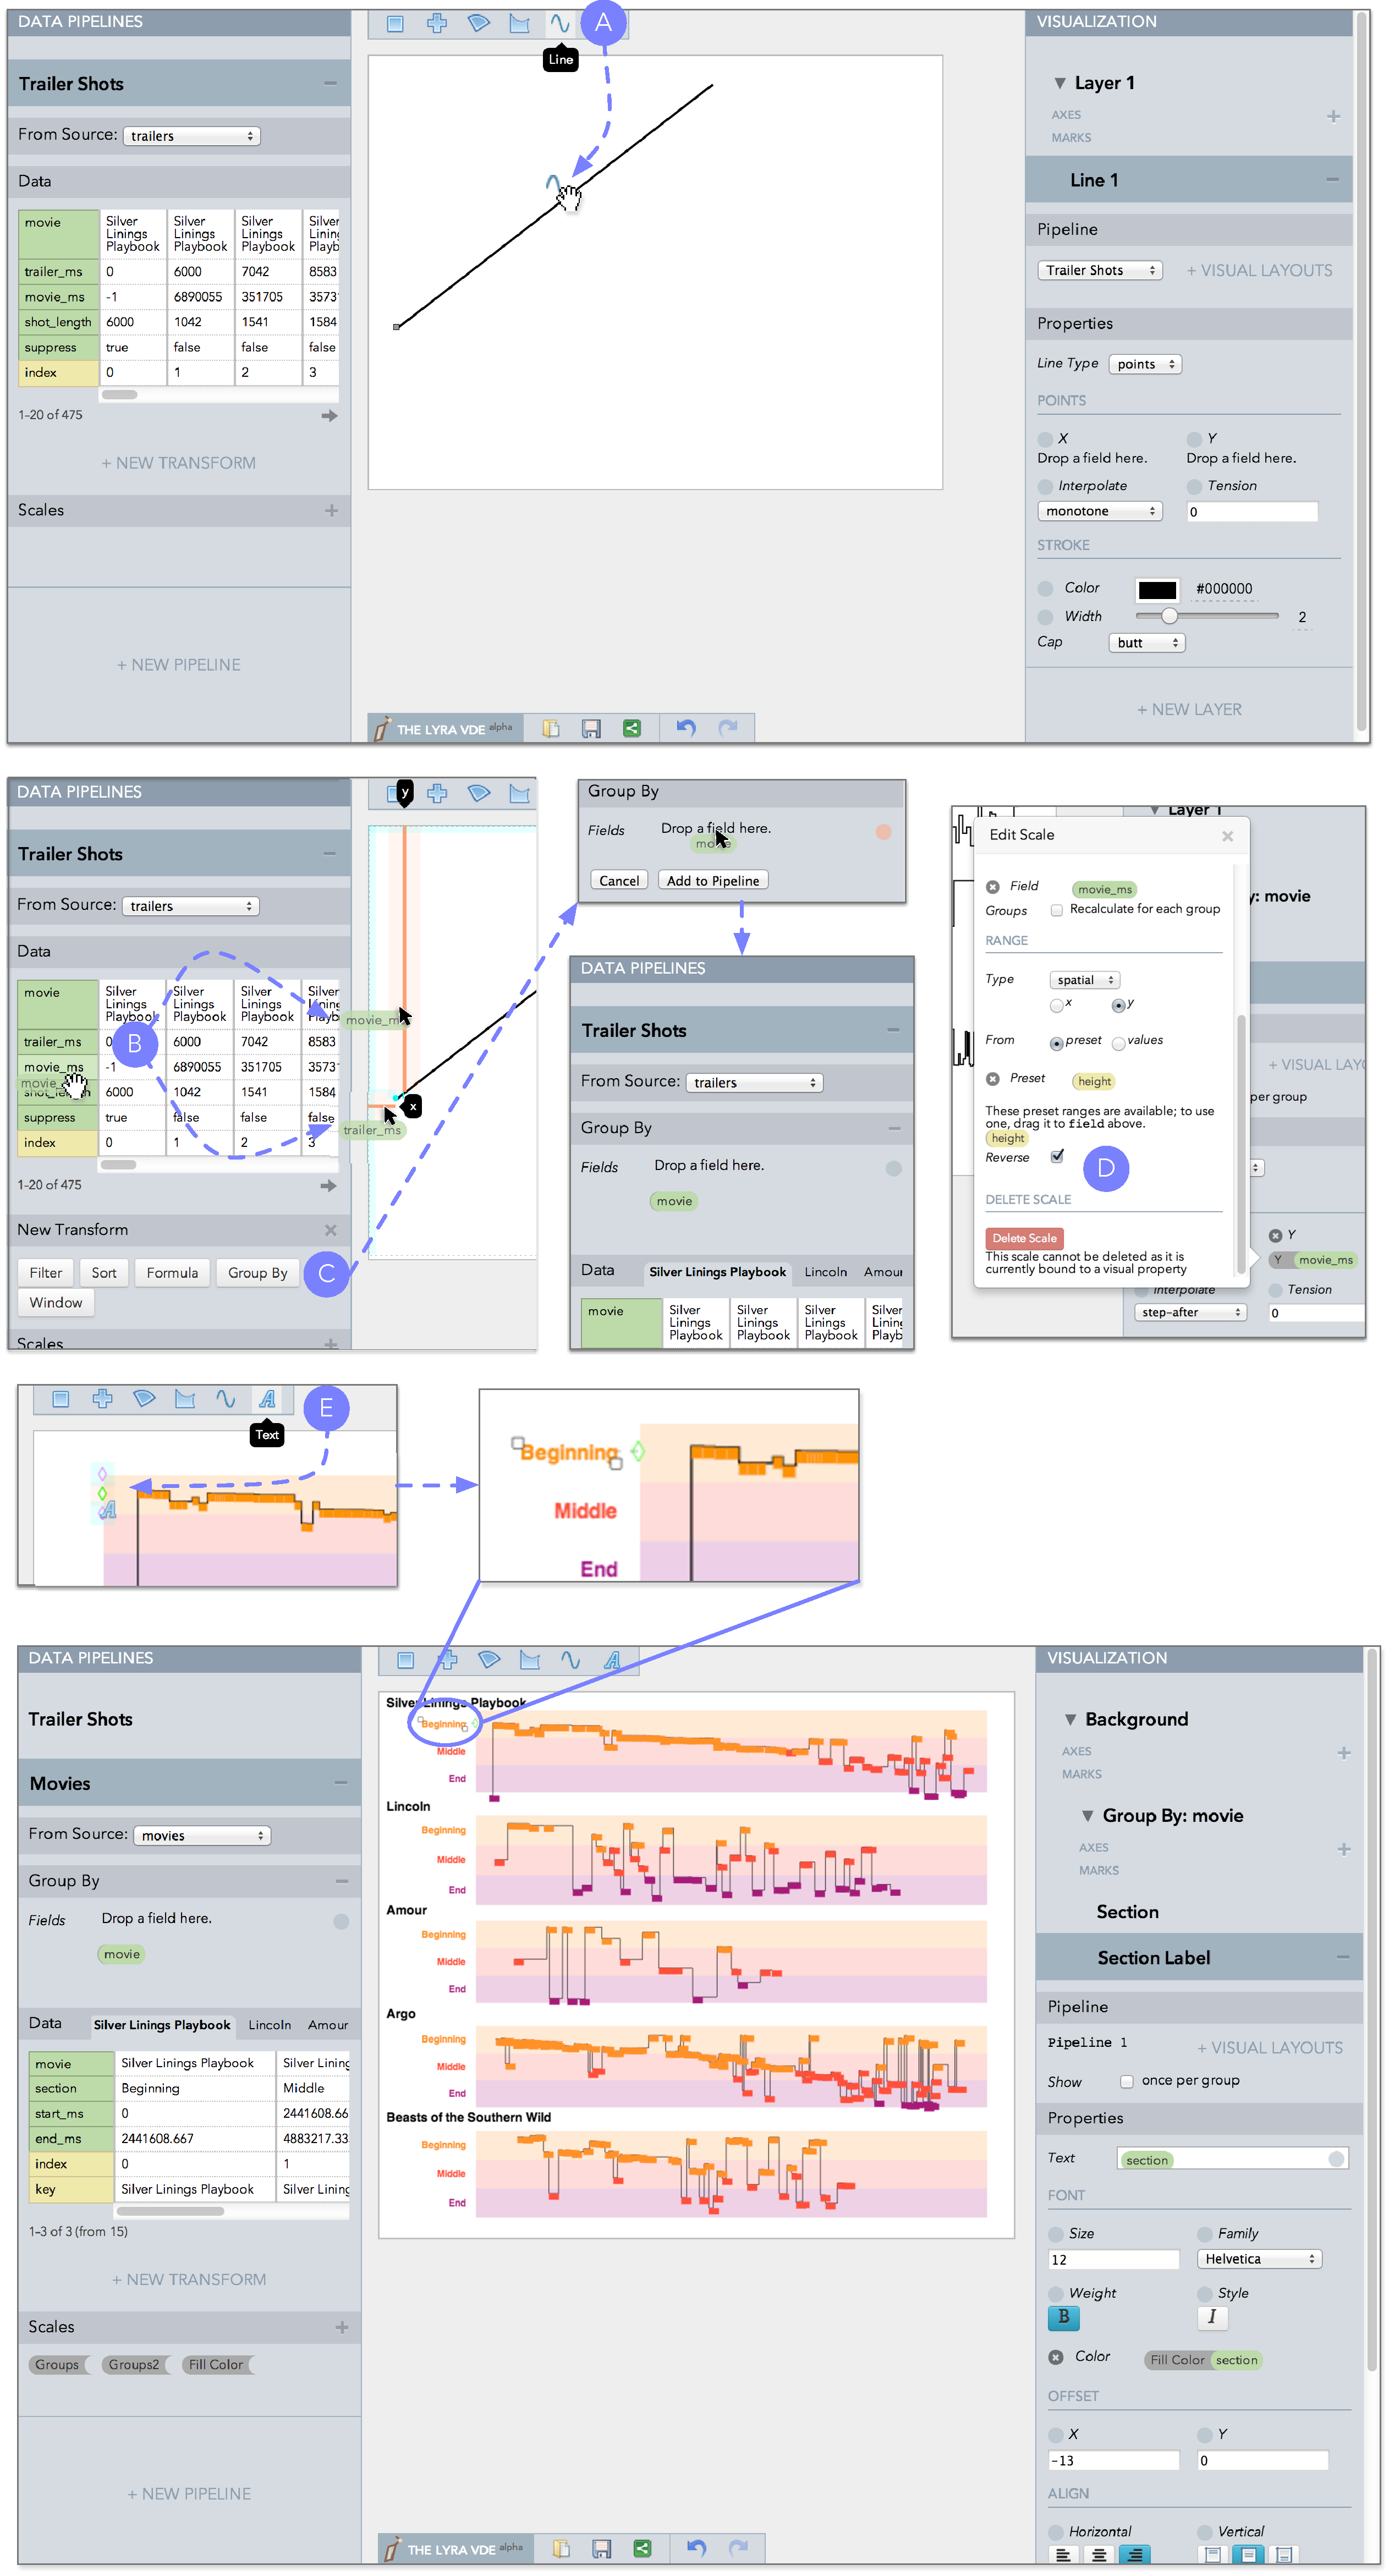
\includegraphics[width=0.7\textwidth]{usage}}
\end{figure}

We introduce lines by dragging a \emph{line mark} from the palette at the top of
the screen and dropping it on the canvas (Fig.~\ref{fig:lyra:usage}(a)). This
adds a new line (backed by a single datum) to the current layer and associates
it with a new data pipeline. The default pipeline is empty, as we have not yet
specified a data source. To register a new source, we provide a name and a URL
to our trailer shots data, and, upon load, review the inferred data types
(number, string, etc.) for each data field. The output of the pipeline is then
shown in the data table at the bottom of the pipeline inspector
(Fig.~\ref{fig:lyra:usage}(b)).

We bind data in the pipeline to visual properties of the line mark via
drag-and-drop of data fields. Dragging triggers the display of \emph{drop zones}
overlaid on the visualization canvas. Dropping a data field on a zone
establishes a visual encoding (Fig.~\ref{fig:lyra:usage}(b)). We drag
\texttt{trailer\_ms} and drop it over the line's \texttt{x} property, then drop
\texttt{movie\_ms} over \texttt{y}. These actions result in line segments
connecting every data point.

However, we desire separate line charts per film. To divide the data, we add a
\emph{group by} transformation to our pipeline (Fig.~\ref{fig:lyra:usage}(c)),
keyed on the movie title. The data table reflects the result via tabbed groups,
and the mark's property inspector now offers an option for group
\texttt{layout}. We choose a \texttt{vertical} layout to produce one line per
movie, arrayed down the canvas. We now see that the data includes shots that
appear in trailers but not in movies (identified by the \texttt{suppress}
field); we add a \emph{filter} transform to remove them
(Fig.~\ref{fig:lyra:usage}(d)). Next, we want film timelines oriented
top-to-bottom, but our lines show the reverse. We adjust the orientation of the
y-axis \emph{scale} by reversing its scale range (Fig.~\ref{fig:lyra:usage}(e)).

Next, we add small rectangle plots by dragging a \emph{rectangle mark} onto the
canvas. Lyra automatically associates the mark with the current pipeline and the
visualization now shows one rectangle per shot. As with the line mark, we drag
\texttt{trailer\_ms} and \texttt{movie\_ms} to the rectangle's \texttt{x} and
\texttt{y} property drop zones. We size the rectangles by dragging
\texttt{shot\_length} over the \texttt{width} drop zone and dragging the bottom
\emph{handle} to manually set the desired height (Fig.~\ref{fig:lyra:usage}(f)).
To color rectangles based on shot onset time in the film, we drag
\texttt{movie\_ms} over the \texttt{fill} property drop zone, and choose custom
colors in the resulting scale definition dialog.

The final step is to create labels and background rectangles to identify the
movies and their beginning, middle, and end sections. As these elements should
reside in the background, we create a new layer in Lyra. Movie section
information is drawn from a different data source, so we create a new pipeline.
We then drag a rectangle mark onto the canvas, and drag the section
\texttt{start} and \texttt{end} fields onto the rectangle \texttt{y} and
\texttt{y2} properties, resulting in a vertical layout for beginning, middle,
and end sections. We bind the \texttt{label} field to the fill color property
and select custom colors for the resulting scale mapping. To label each section,
we drag a \emph{text mark} from the palette and drop it on a rectangle's
diamond-shaped \emph{connector} (Fig.~\ref{fig:lyra:usage}(g)). Doing so anchors
the text mark coordinates to the rectangle. Finally, we bind the \texttt{label}
field as textual content and set the text fill color. We now can export the
visualization as either a Vega specification or an image file.